A continuación se describen detalladamente cómo se han ejecutado los experimentos para cada algoritmo, empleando el mismo esquema de ejecución.

Las ejecuciones realizadas en este trabajo de investigación han sido realizadas usando la herramienta Jypyter notebook \cite{ProjectHome}. Gracias a ésta se han publicado los resultados obtenidos durante de las ejecuciones de los experimentos  junto con el código implementado para cada modelo. 

En el repositorio Github de este trabajo bajo directorio 'examples' (\url{https://github.com/efrain70/NeuDataLoad/tree/master/examples/notebooks}) se ecuentran todas las ejecuciones realizadas para los modelos seleccionados.

\section{Sistema para la ejecución}
La ejecución de los experimentos se ha ejecutado en un ordenador personal, con Ubuntu 16.04.2 como sistema operativo con CUDA \cite{ProcesamientoNVIDIA} instalado y la siguiente configuración de hardware:
\begin{itemize}
    \item Tarjeta gráfica NVIDIA® GeForce® GTX 1050 (4 GB GDDR5 dedicados)
    \item Procesador Intel® Core™ i7-7700HQ (2.8, 3.8GHz, 6 MB Cache, 4 núcleos, 8 hijos de procesamiento)
    \item Memoria DDR4-2133 SDRAM, 16 GB (2 x 8 GB)
    \item Almacenamiento 1 TB HDD,  256 GB SSD
\end{itemize}

\section{Carga de los datos}
Este es el momento cuando se cargan todos los datos provenientes de los ficheros y la hoja de cálculo. En la imagen \ref{figure:codeload} podemos ver como la la salida de la ejecución muestra los errores al realizar la validación de los datos y el código de su ejecución. En este caso concreto, se encuentran las 40 matrices que no disponen de su elemento correspondiente en el índice principal.

\begin{figure}[H]
\centering
\fbox{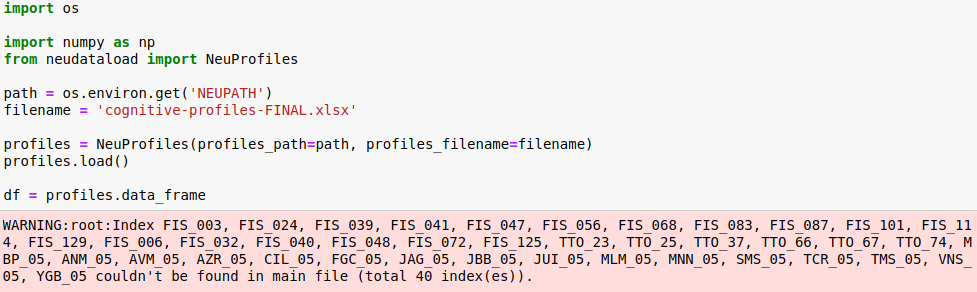
\includegraphics[width=0.85\textwidth]{figs/ejecucion/code_load.png}}
\caption{Código y resultado de ejecución para la carga de los datos.}
\label{figure:codeload}
\end{figure}


\section{Selección de los ejemplares}
Como se aprecia en la tabla \ref{table:totales} hay ejemplares que no tienen algunas matrices de adyacencia. Por este motivo, se han repetido las ejecuciones de cada algoritmo dos veces; para los que tienen todas las matrices y para los que tienen todas las matrices relacionadas con \gls{dti} (FA, L1, MD y RX). El código para este caso se expone en la imagen \ref{figure:codeselect}.

\begin{figure}[H]
\centering
\fbox{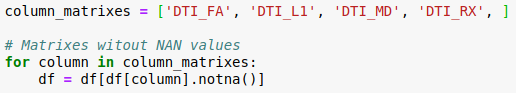
\includegraphics[width=0.6\textwidth]{figs/ejecucion/code_seleccion.png}}
\caption{Código para la selección de las matrices \gls{dti}.}
\label{figure:codeselect}
\end{figure}


\section{Configuración de las etiquetas}
Como se ha comentado en la sección \ref{section:distdatos}, la clase binaria objetivo, memoria, se encuentra descrita en el atributo ``profile'' de la hoja del cálculo. En base a los valores, se establece su valor correspondiente usando el código de la imagen \ref{figure:codelabel}. Un ejemplo de cómo quedan estos valores se aprecia en la imagen \ref{figure:outlabel}.

\begin{figure}[H]
\centering
\fbox{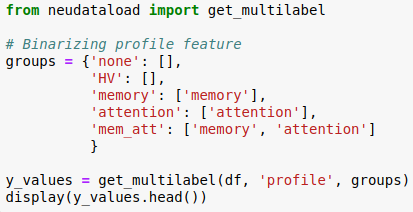
\includegraphics[width=0.5\textwidth]{figs/ejecucion/code_etiquetas.png}}
\caption{Código para obtención de las etiquetas.}
\label{figure:codelabel}
\end{figure}

\begin{figure}[H]
\centering
\fbox{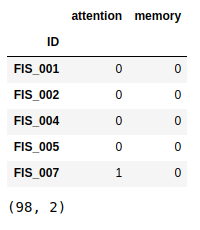
\includegraphics[width=0.35\textwidth]{figs/ejecucion/outout_labels.png}}
\caption{Resultado de las etiquetas de las primeras instancias.}
\label{figure:outlabel}
\end{figure}

\section{Conjunto de entrenamiento y test}
Con los valores de las instancias con sus respectivas etiquetas se aplica el algoritmo para la separación de los conjuntos de entrenamiento y test (ver \ref{section:validacion}). Se ha separado un 20\% de la muestra para el test y el resto para el entrenamiento (imagen \ref{figure:traintest}).

\begin{figure}[H]
\centering
\fbox{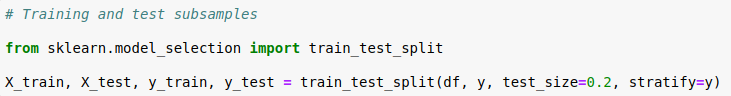
\includegraphics[width=0.8\textwidth]{figs/ejecucion/code_traintest.png}}
\caption{Código para la aplicación de \gls{kfold}.}
\label{figure:traintest}
\end{figure}

\section{Selección de la configuración}
Cada algoritmo tiene su parámetros propios configurables y sus configuraciones para el preprocesado pueden ser distintas. Para definir cada una de ellas se han implementado ``pipelines'' que definen el flujo de ejecución. Estos son ejecutados usando nuevamente una separación de los conjuntos de entrenamiento y validación (ver sección \ref{section:validacion}). Otro punto importante es cómo se comparan los resultados de las configuraciones, en nuestro caso se ha optado por la más general, nivel de acierto de las etiquetas.

\subsection{Logistic Regression}
Para este algoritmo se han configurado los parámetros ``penalty'' y ``C'', imagen \ref{figure:paramlog}:
\begin{description}
    \item [Penalty]  tipo de penalización.
    \item [C] coeficiente de regulación.
\end{description}

\begin{figure}[H]
\centering
\fbox{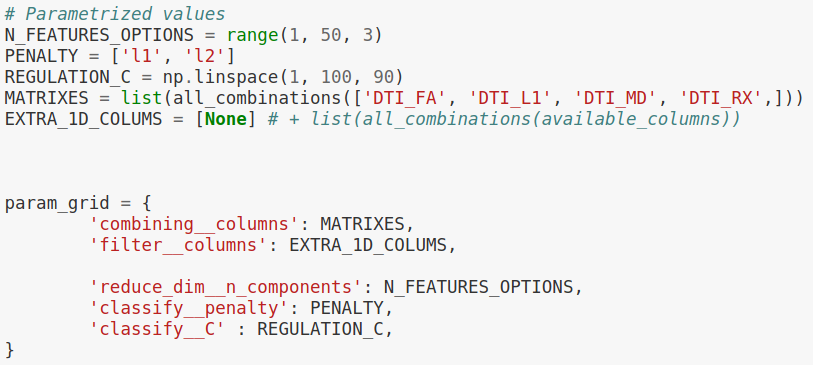
\includegraphics[width=0.8\textwidth]{figs/ejecucion/code_param_log.png}}
\caption{Código para la selección de parámetros de Logistic Regression.}
\label{figure:paramlog}
\end{figure}

\subsection{Support Vector Machine}
Los parámetros para este algoritmo son, ``degree'' y ``C'', imagen \ref{figure:paramsvm}:
\begin{description}
    \item [Degree] Grado del hiperplano.
    \item [C] Grado de penalización por error.
\end{description}

\begin{figure}[H]
\centering
\fbox{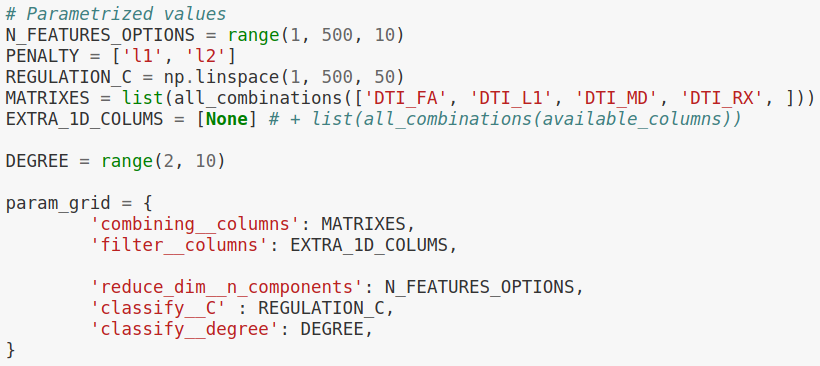
\includegraphics[width=0.8\textwidth]{figs/ejecucion/code_param_svm.png}}
\caption{Código para la selección de parámetros de Support Vector Machine.}
\label{figure:paramsvm}
\end{figure}

\subsection{Gaussian Naive Bayes}
Para este algoritmo no se ha configurado ningún parámetro durante la búsqueda, imagen \ref{figure:parambayes}.

\begin{figure}[H]
\centering
\fbox{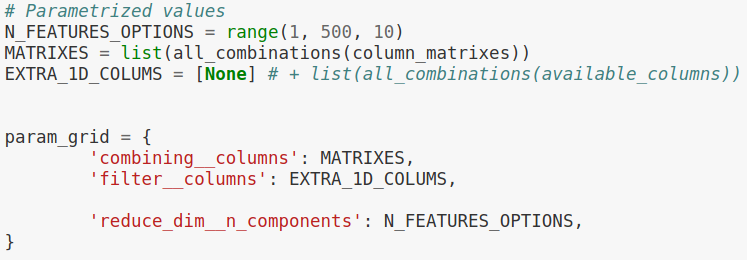
\includegraphics[width=0.8\textwidth]{figs/ejecucion/code_param_bayes.png}}
\caption{Código para la selección de parámetros de Gaussian Naive Bayes.}
\label{figure:parambayes}
\end{figure}

\subsection{Random Forest Classifier}
El parámetro que configura este algoritmo es ``max\_depth'', imagen \ref{figure:paramforest}:
\begin{description}
    \item [max\_depth] Profundidad máxima de los árboles.
\end{description}

\begin{figure}[H]
\centering
\fbox{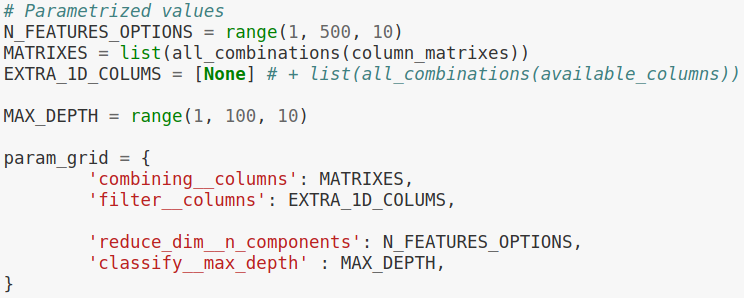
\includegraphics[width=0.8\textwidth]{figs/ejecucion/code_param_forest.png}}
\caption{Código para la selección de parámetros de Random Forest Classifier.}
\label{figure:paramforest}
\end{figure}


\subsection{Artificial Neural Network}
Este algoritmo puede ser el más difícil de configurar al ser el más complejo. Usando una red neuronal bastante simple con una única capa oculta. En la imagen \ref{figure:designann} se puede ver cómo se ha diseñado y en \ref{figure:paramann} los parámetros:
\begin{description}
 \item [n\_hidden] Número de células en la capa oculta.
 \item [learning\_rate] Grado de aprendizaje de la red neuronal.
 \item [epochs] Épocas de entrenamiento de la red neuronal.
\end{description}

\begin{figure}[H]
\centering
\fbox{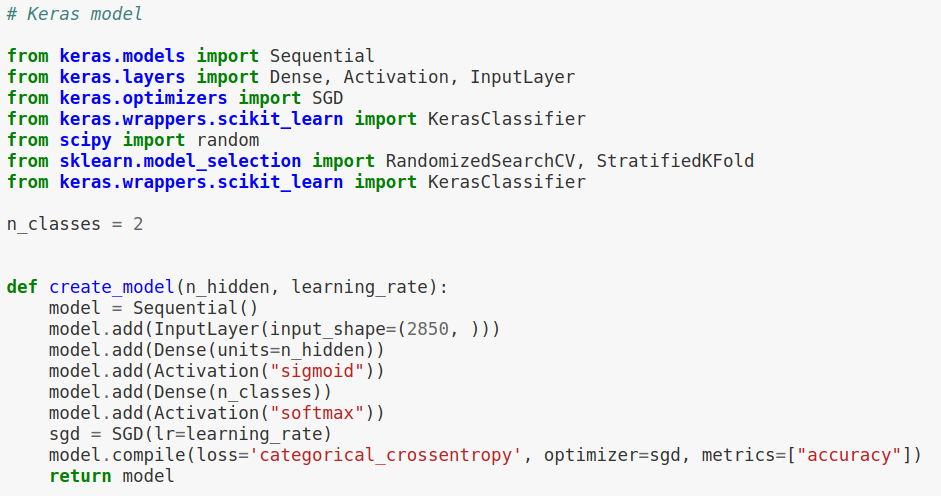
\includegraphics[width=0.8\textwidth]{figs/ejecucion/code_design_ann.png}}
\caption{Código para el diseño del modelo de Artificial Neural Network.}
\label{figure:designann}
\end{figure}

\begin{figure}[H]
\centering
\fbox{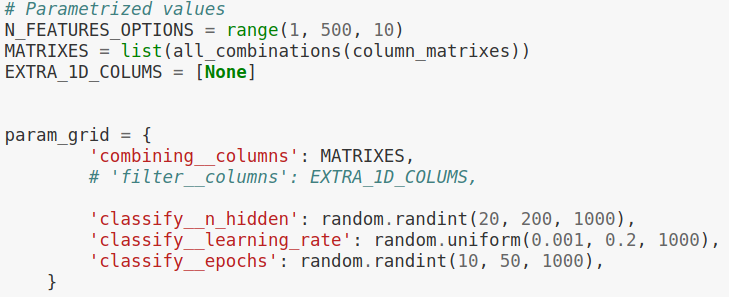
\includegraphics[width=0.8\textwidth]{figs/ejecucion/code_param_ann.png}}
\caption{Código para la selección de parámetros de Artificial Neural Network.}
\label{figure:paramann}
\end{figure}